\section{Mathematical optimisation}
Optimisation is a way to find out the best solution to the problem. The starting point for optimisation is to define an objective function or the cost function. For an objective function $f: A \rightarrow  \mathbb{R}$, the goal of optimisation is to find $x_0 \in A$ such that $f(x_0) \leq f(x)$ $\forall\ x \in A$. If the objective function is differentiable, then we can use the gradient information to reach the optimal point. Non differentiable functions are usually optimised by heuristic optimisation methods. Heuristic methods often provide a near optimal solution even if the search space is large. The following optimisation methods are used in this study.


\subsection{Simulated annealing}
\label{subsection:sim_anneal}
Simulated annealing is a heuristic optimisation technique inspired by the way metals cool and anneal. More precisely, it is based on the thermodynamics of a system undergoing a slow cooling so that the atoms have sufficient time to redistribute to form a crystalline structure\textemdash a state of minimum energy  \cite{Kirkpatrick1983-hh, Ingber2000-aw, Keith2002-jx, Brownlee2011-bk, presse1988numerical}. This algorithm is often used to solve combinatorial optimisation problems in bioinfomatics and other sciences. It has been used to align and predict non-coding RNAs from multiple sequences \cite{Lindgreen2007-jy}, to find consensus sequences \cite{Keith2002-jx} and optimise the ribosome binding sites \cite{Salis2009-dh} and mRNA folding using minimum free energy models \cite{Gaspar2013-bg}.

Let $p_i$ be the probability that a system is in a certain state $i$ with energy $\epsilon_i$. Then entropy of the system is defined as:
\begin{equation}
    S = -k_B\sum_{i} p_i \ln(p_i)
    \label{eqn:entropy}
\end{equation}
where $k_B$ is the Boltzmann's constant. For any system, the second law of thermodynamics states that the entropy is maximised as the system evolves towards a  thermodynamic equilibrium. Hence, to know the behaviour of the system, Equation \ref{eqn:entropy} needs to be maximised under these two constrains:
\begin{equation}
    \begin{split}
        1)\ \sum_j p_j &= 1 \\
        2)\ \sum_j p_j \epsilon_j &= E
    \end{split}
\end{equation}
The first condition simply means that sum of all probabilities should be one while the second condition implies the total energy of the system is a constant $E$. Using Lagrange multipliers,  
\begin{equation}
    S = -k_B\sum_j p_j \ln(p_j) - \lambda [\sum_j p_j -1 ] - \beta[\sum_j p_j \epsilon_j - E]
    \label{eqn:lagrange_mult}
\end{equation}
Setting the first derivative of Equation \ref{eqn:lagrange_mult} to zero, we obtain:
\begin{equation}
    p_i = e^{1-\lambda}.e^{-\beta \epsilon_i}
    \label{eqn:prob_aft_max}
\end{equation}
$\beta$, also known as thermodynamic beta, can be shown to be equal to $1/k_B T$, where $T$ is the absolute temperature. $\lambda$ is chosen to normalise the probability $p_i$ in Equation \ref{eqn:prob_aft_max}. We thus arrive at the Boltzmann's probability distribution:
\begin{equation}
    p_i = \frac{1}{Z} e^{-\beta \epsilon_i}
    \label{eqn:prob_boltzmann}
\end{equation}
where $Z$ is the partition function. For a system in thermal equilibrium at temperature $T$, Equation \ref{eqn:prob_boltzmann} gives us a set of probability mass functions for all different energy states $\epsilon_i$. An interesting implication of the Boltzmann's distribution is that even at low temperature, there is a non zero probability of system being at high energy.  


A mathematical way to reach the minima of the Boltzmann's distribution is by using a Markov chain sampling while simultaneously decreasing the temperature. The decreasing temperature is simulated by applying a cooling schedule, which is generally exponentially decreasing \cite{Kirkpatrick1983-hh}. Markov chain sampling can be performed by using the Metropolis-Hastings algorithm or perhaps Gibb's sampling, although this is less commonly used  \cite{Keith2002-jx}. For the Metropolis-Hastings algorithm, a \textit{bad} move (uphill) $E_2$ from initial state $E_1$ such that $E_2 > E_1$, is accepted if $R(0,1) \geq p_2/p_1$, where $R(0,1)$ is a uniformly generated random number between $0$ and $1$ \cite{hastings1970monte}. Unlike gradient descent, where only \textit{good} moves (downhill) ($E_2 < E_1)$ are accepted, this algorithm can move both uphill and downhill without getting trapped in any local minima. The probability of system moving uphill, however, decreases with temperature \cite{presse1988numerical}. 


%‘bad’ move
A use case of simulated annealing on a Rastrigin function (a test function commonly used to to demonstrate optimisation) (Figure \ref{fig:rastrigin}) is shown in Figure \ref{fig:sim_anneal}. 

\begin{figure}[H]
\center
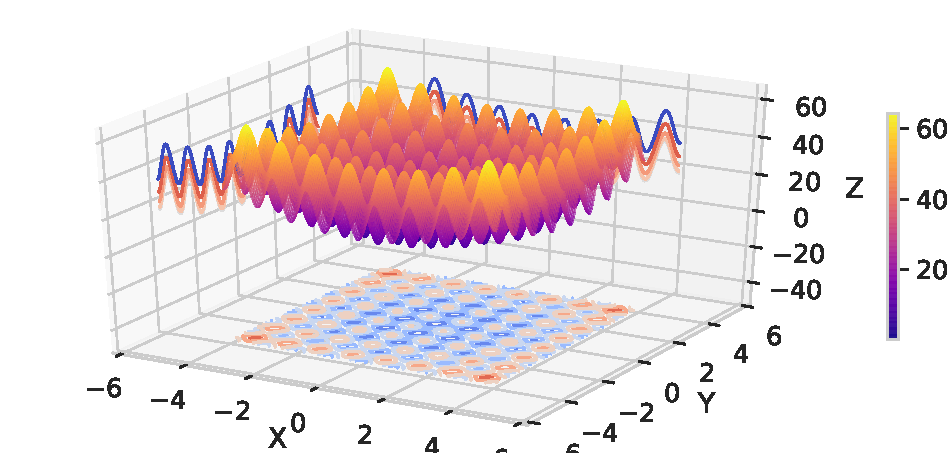
\includegraphics[width=1\textwidth]{chapters/Introduction/Figures/rastrigin.pdf}
\caption[Two dimensional Rastrigin function.]{\textbf{Two dimensional Rastrigin function.} Rastrigin function is frequently used as a test function in optimisation problems because of a large number of local minima. The global minima is at $(0, 0)$ where the value of function is $0$.}%the List of Figures because of the *}
\label{fig:rastrigin}
\end{figure}


\begin{figure}[H]
\center
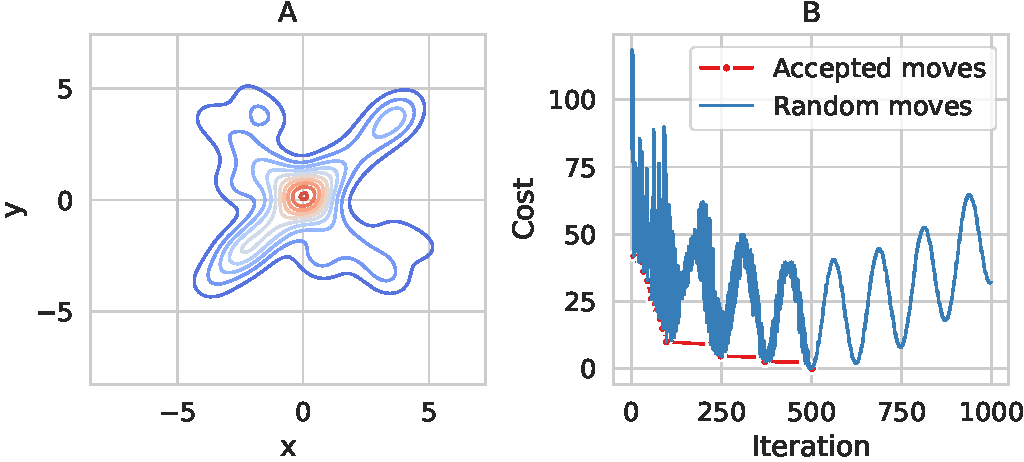
\includegraphics[width=1\textwidth]{chapters/Introduction/Figures/simulated_annealing.pdf}
\caption[Simulated annealing on a two dimensional Rastrigin function.]{\textbf{Simulated annealing on a two dimensional Rastrigin function.} This simulation was run for $1,000$ iterations with an initial temperature of $1$. The minimum found was at $(0.006, -0.013)$, where the value of function was $0.04$.  \textbf{(A)} Kernel density estimate of the moves during simulated annealing shows that they converge near the true minimum $(0, 0)$. \textbf{(B)} The accepted costs are usually immune to the traps of local minima. The algorithm converted at $502^{nd}$ iteration, where the accepted cost is $0.04$. This is close to the global minima $0$. }%the List of Figures because of the *}
\label{fig:sim_anneal}
\end{figure}


\subsection{Nelder-Mead method}
The Nelder-Mead method is another type of derivative-free, heuristic optimisation technique \cite{Nelder1965-zb}. The method, however, requires the objective function to be evaluated at different points hence can also be categorised as a \textit{direct search} method. Direct search methods usually employ a non-degenerate simplex at each step \cite{lagarias1998convergence}. Simplex in $n$ dimensions is a convex-hull of $n+1$ vertices and can be understood as a generalisation of triangles. By non-degenerate, we mean the volume of the simplex is non zero.

% \footnote{Simplex in $n$ dimensions is a convex-hull of $n+1$ vertices and can be understood as a generalisation of triangles. By non-degenerate, we mean the volume of the simplex is non zero.}

For an $n$ dimensional function $f(x)$, initialisation is performed by choosing $n+1$ points $(x_i, 1\leq i \leq n+1)$ which form a simplex. These points are ordered such that $f(x_1) \leq f(x_2) \leq ... f(x_{n+1})$. Since the goal is to minimise $f(x)$, in this case $x_{n+1}$ is the worst point and $x_1$ is the best. The worst point is then reflected along the centroid of the simplex to give a new vertex $x_r$ such that the volume is preserved and the non-degeneracy is maintained \cite{presse1988numerical}. Three cases may happen:

\begin{itemize}
  \item $f(x) \leq f(x_r) \leq f(x_{n+1})$
  
  In this case, the new move is neither good nor bad. $x_r$ replaces some older point $x_o$ where $f(x) \leq f(x_o) \leq f(x_{n+1})$.
  
  \item $f(x) \leq f(x_{n+1}) \leq f(x_r) $
  
  In this case, the new move is worse. The simplex is contracted by decreasing $x_{n+1}$ to $x_c$. If $x_c < Min(f(x_{n+1}), f(x_r))$, $x_{n+1}$ is replaced by $x_c$. Else, contraction is repeated.
  
  \item $f(x_r) \leq f(x_1) \leq f(x_{n+1}) $
  
  In this case, the new move is good. $x_r$ replaces the older best point $x_1$. 
\end{itemize}

The ordering of points and reflection are repeated, until the change in the value of the function at the best point falls below a preset tolerance. This method tends to get stuck at local minima (Figure \ref{fig:nelder-mead} A, B), because whenever it encounters one, the algorithm contracts the simplex rather than exploring the surrounding. However for functions with a few or no local minima, for example, Rosenbrock function (Fig. \ref{fig:rosen}), if the starting point is good, this algorithm is very efficient in finding the minima (which is often global) (Figure \ref{fig:nelder-mead} C, D).


\begin{figure}[H]
\center
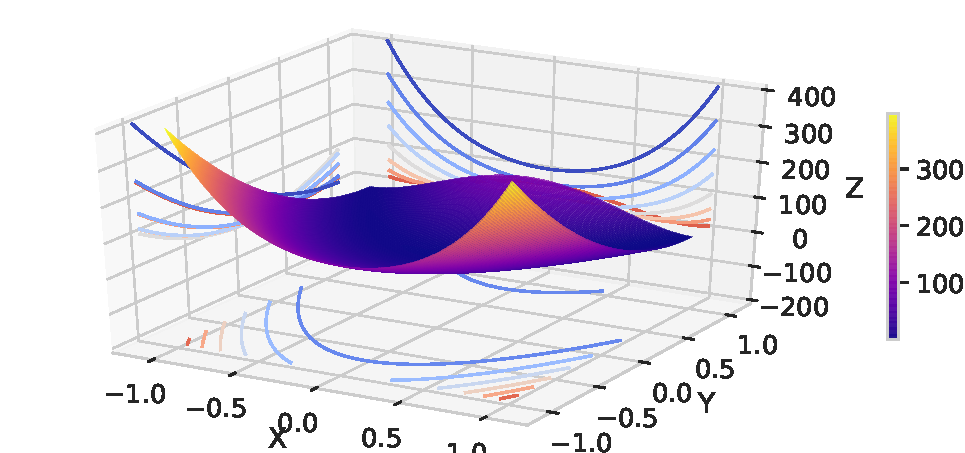
\includegraphics[width=0.75\textwidth]{chapters/Introduction/Figures/rosen.pdf}
\caption[Two dimensional Rosenbrock function.]{\textbf{Two dimensional Rosenbrock function.} Rosebrock function is a test function often used to demonstrate optimisation. It has a characteristic valley where the global minimum lies. The global minima is at $(1, 1)$ where the value of function is $0$.}%the List of Figures because of the *}
\label{fig:rosen}
\end{figure}

\begin{figure}[H]
\center
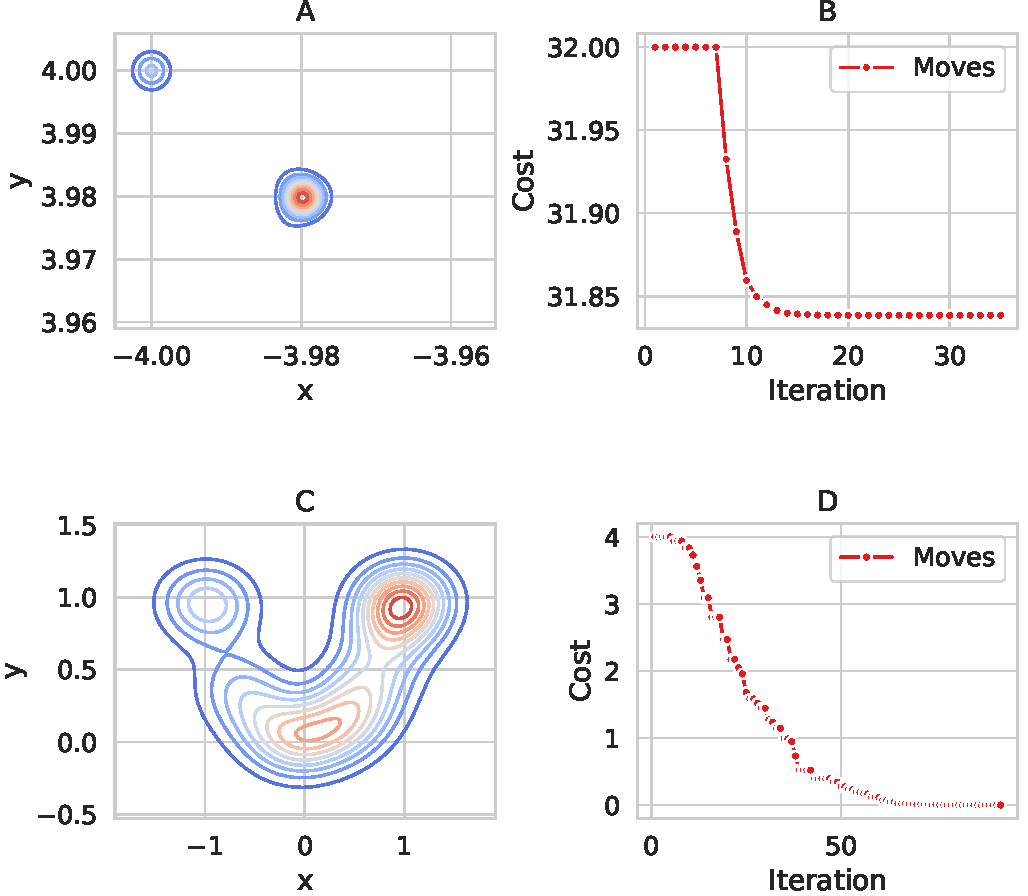
\includegraphics[width=0.75\textwidth]{chapters/Introduction/Figures/Nelder-Mead.pdf}
\caption[Although the Nelder-Mead method tends to get stuck on local minima, a good initial point can result in a global optimum.]{\textbf{Although the Nelder-Mead method tends to get stuck on local minima, a good initial point can result in a global optimum.} \textbf{(A)} Nelder-Mead method applied on a Rastrigin function. Rastrigin function is a test function often used to demonstrate optimisation. Kernel density estimate of the moves shows that the algorithm gets stuck at a local minima $(-3.98, 3.98)$. \textbf{(B)} The algorithm terminated after $35$ iterations where the minimum was found to be $3.36$, which is a local minimum. \textbf{(C)} Nelder-Mead method applied on a Rosenbrock function with $(-2,2)$ as the starting point. Kernel density estimate of the moves shows that the algorithm moves around the valley and terminates at $(1.0001, 1.0002)$ close to the global minima. \textbf{(D)} The algorithm terminated after $92$ iterations where the minimum was found to be $3.36 \times 10^{-8}$.}%the List of Figures because of the *}
\label{fig:nelder-mead}
\end{figure}